% Results. Every number is a macro from generated/numbers.tex (written by `run.py report` from results/), and every
% table is generated from the same files; no number in this file is typed by hand.

\subsection{Synthetic test set}
Table~\ref{tab:results} compares all systems. On the full test set ($n=\nMethod$ clouds), the method selects the correct family for \accMethod{} \accCIMethod{} of the clouds, with a median Chamfer distance to the noise-free ground-truth shape of \cdMethod{} \cdCIMethod{} (in units of the RMS radius of the cloud). On the baseline subset, where every system sees the same $n=\nBone$ clouds, the method reaches \accMethodsub{}, against \accBtwo{} for the feature classifier B2, \accBone{} for the classical fit-every-family pipeline B1, and \accBthreea{}--\accBthreec{} for the trivial baselines.

\begin{table}[tbp]
\centering
\caption{Synthetic test set. Fine accuracy is the exact family; coarse accuracy is the shape dimension (point set, curve, surface, blob). Chamfer is the median symmetric Chamfer distance between the selected, refined shape and the noise-free ground-truth shape. Baselines and the ``baseline subset'' row use the same 20 clouds per family and cell. 95\% percentile-bootstrap CIs. The full table (superset-tolerant accuracy, residual, axis error) is in \texttt{reports/exp01\_synthetic.md}.}
\label{tab:results}
\resizebox{\textwidth}{!}{\scriptsize
\begin{tabular}{llllll}
\toprule
\textbf{System} & \textbf{n} & \textbf{Fine accuracy [95\% CI]} & \textbf{Macro-F1 [95\% CI]} & \textbf{Coarse accuracy} & \textbf{Median Chamfer to GT [95\% CI]} \\
\midrule
Method (network + refinement) & 39000 & 87.9\% [87.6, 88.2] & 0.879 [0.876, 0.882] & 92.7\% & 0.156 [0.154, 0.158] \\
Method, baseline subset & 3120 & 87.4\% [86.2, 88.5] & 0.873 [0.862, 0.884] & 92.3\% & 0.154 [0.147, 0.161] \\
A3: no refinement & 39000 & 87.9\% [87.6, 88.2] & 0.879 [0.876, 0.882] & 92.7\% & 0.159 [0.157, 0.162] \\
A5: G-AIC selection & 39000 & 64.6\% [64.1, 65.1] & 0.627 [0.623, 0.632] & 77.5\% & 0.182 [0.179, 0.185] \\
A5: hybrid selection & 39000 & 85.6\% [85.2, 85.9] & 0.858 [0.854, 0.861] & 91.1\% & 0.157 [0.155, 0.159] \\
B1: classical fit + G-AIC & 3120 & 52.2\% [50.6, 54.0] & 0.499 [0.484, 0.515] & 70.7\% & 0.209 [0.200, 0.221] \\
B2: features + boosting & 3120 & 64.5\% [62.8, 66.2] & 0.645 [0.629, 0.662] & 85.1\% & 0.237 [0.221, 0.255] \\
B3a: always blob & 3120 & 7.7\% [6.8, 8.7] & 0.011 [0.010, 0.012] & 7.7\% & 0.543 [0.536, 0.550] \\
B3b: always circle & 3120 & 7.7\% [6.8, 8.6] & 0.011 [0.010, 0.012] & 38.5\% & 0.545 [0.536, 0.555] \\
B3c: random shape & 3120 & 7.9\% [7.1, 8.8] & 0.079 [0.070, 0.088] & 32.9\% & 1.116 [1.100, 1.137] \\
\bottomrule
\end{tabular}
}
\end{table}

\paragraph{Preregistered hypotheses (Table~\ref{tab:hypotheses}).} H1 is supported: the paired macro-F1 difference between the method and B1 is \estHone{} \ciHone{}. H2 is supported: the paired difference in median Chamfer distance is \estHtwo{} \ciHtwo{}. Refinement (H5b) lowers the median Chamfer distance by a small but significant amount, \estHfivebrefinement{} \ciHfivebrefinement{}; because the family is selected by the classifier before refinement, refinement cannot change accuracy (A3 has the same accuracy as the method by construction). H5a (Chamfer versus parameter-space loss) requires the ablation runs, which are postponed (Sec.~\ref{sec:limitations}).

\begin{table}[H]
\centering
\caption{Preregistered hypotheses. p-values are Holm-corrected over the synthetic comparisons; H3 uses an exact binomial CI and a 10{,}000-permutation null over predicted coarse labels.}
\label{tab:hypotheses}
\resizebox{\textwidth}{!}{\scriptsize
\begin{tabular}{llllll}
\toprule
\textbf{Hypothesis} & \textbf{Comparison} & \textbf{Estimate [95\% CI]} & \textbf{p (Holm)} & \textbf{n} & \textbf{Verdict} \\
\midrule
H1 & macro-F1(method) - macro-F1(B1) & 0.3741 [0.3572, 0.3905] & $<$ 1e-16 & 3120 & supported \\
H2 & median Chamfer(method) - median Chamfer(B1) & -0.0554 [-0.0645, -0.0462] & $<$ 1e-16 & 3120 & supported \\
H5b\_refinement & median Chamfer(method) - median Chamfer(no refinement) & -0.0033 [-0.0046, -0.0021] & $<$ 1e-16 & 39000 & supported \\
H3 & Coarse-label agreement (subsample majority) with literature on preregistered real datasets & 7/12 = 58\% [28, 85] (exact binomial) & perm. p = 0.125 & 12 & not supported \\
H4 & Controls: matched Gaussians $\to$ blob (mean over 17 real datasets); ordinal processes $\to$ ringing (not helix) & blob rate 86\%; ringing 60\% vs helix 40\% & - & - & supported \\
\bottomrule
\end{tabular}
}
\end{table}

\paragraph{Where the gap comes from.} Selecting among the network's own refined candidates with geometric AIC (A5) lowers accuracy to \accAfivegaic{}, close to B2. Model selection, not fitting, is what separates the systems: with nested families and realistic noise a residual-versus-complexity criterion often prefers the more flexible family, while the classifier has learned the prior over families and noise that generated the data. The advantage of the method is largest for the smallest clouds (Fig.~\ref{fig:byn}). The hardest families are cone, helix and paraboloid; most of their errors are confusions with each other (Appendix, Fig.~\ref{fig:confusion}). Temperature scaling with $T=\temperature$ fitted on the validation stream lowers the expected calibration error from \eceBefore{} to \eceAfter{} and the NLL from \nllBefore{} to \nllAfter{} (Appendix, Fig.~\ref{fig:reliability}).

\begin{figure}[tbp]
\centering
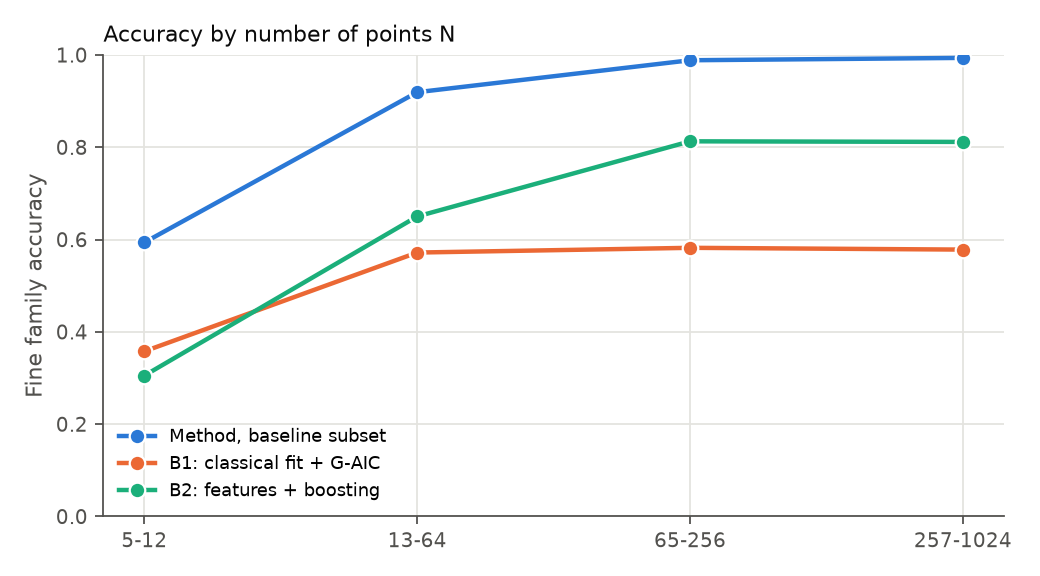
\includegraphics[width=0.48\textwidth]{fig_by_n.png}\hfill
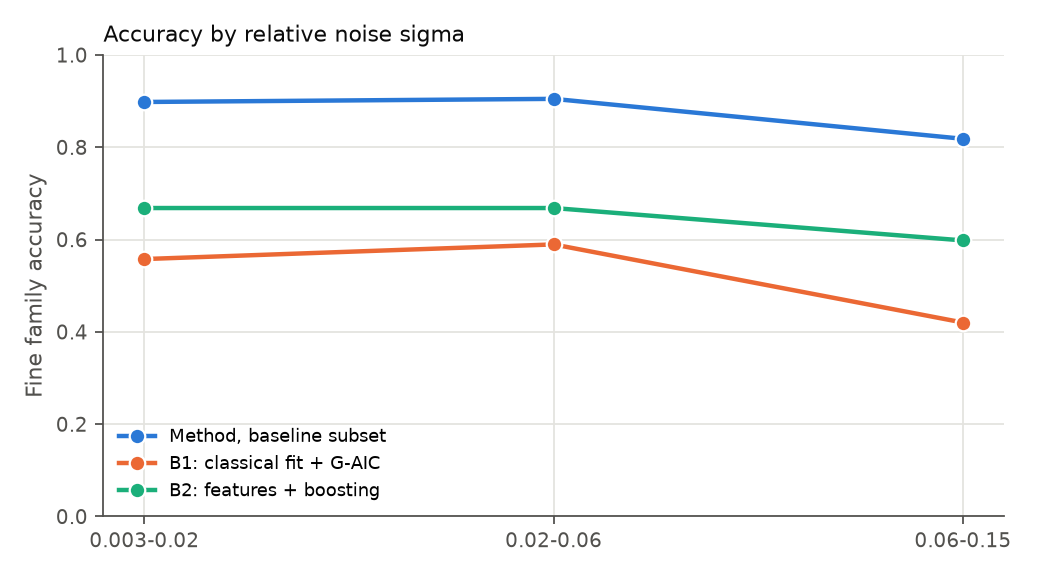
\includegraphics[width=0.48\textwidth]{fig_by_noise.png}
\caption{Fine accuracy by number of points and by relative noise on the baseline subset (the same clouds for every line). A3 is omitted because its accuracy equals the method's by construction.}
\label{fig:byn}
\end{figure}

\begin{figure}[tbp]
\centering
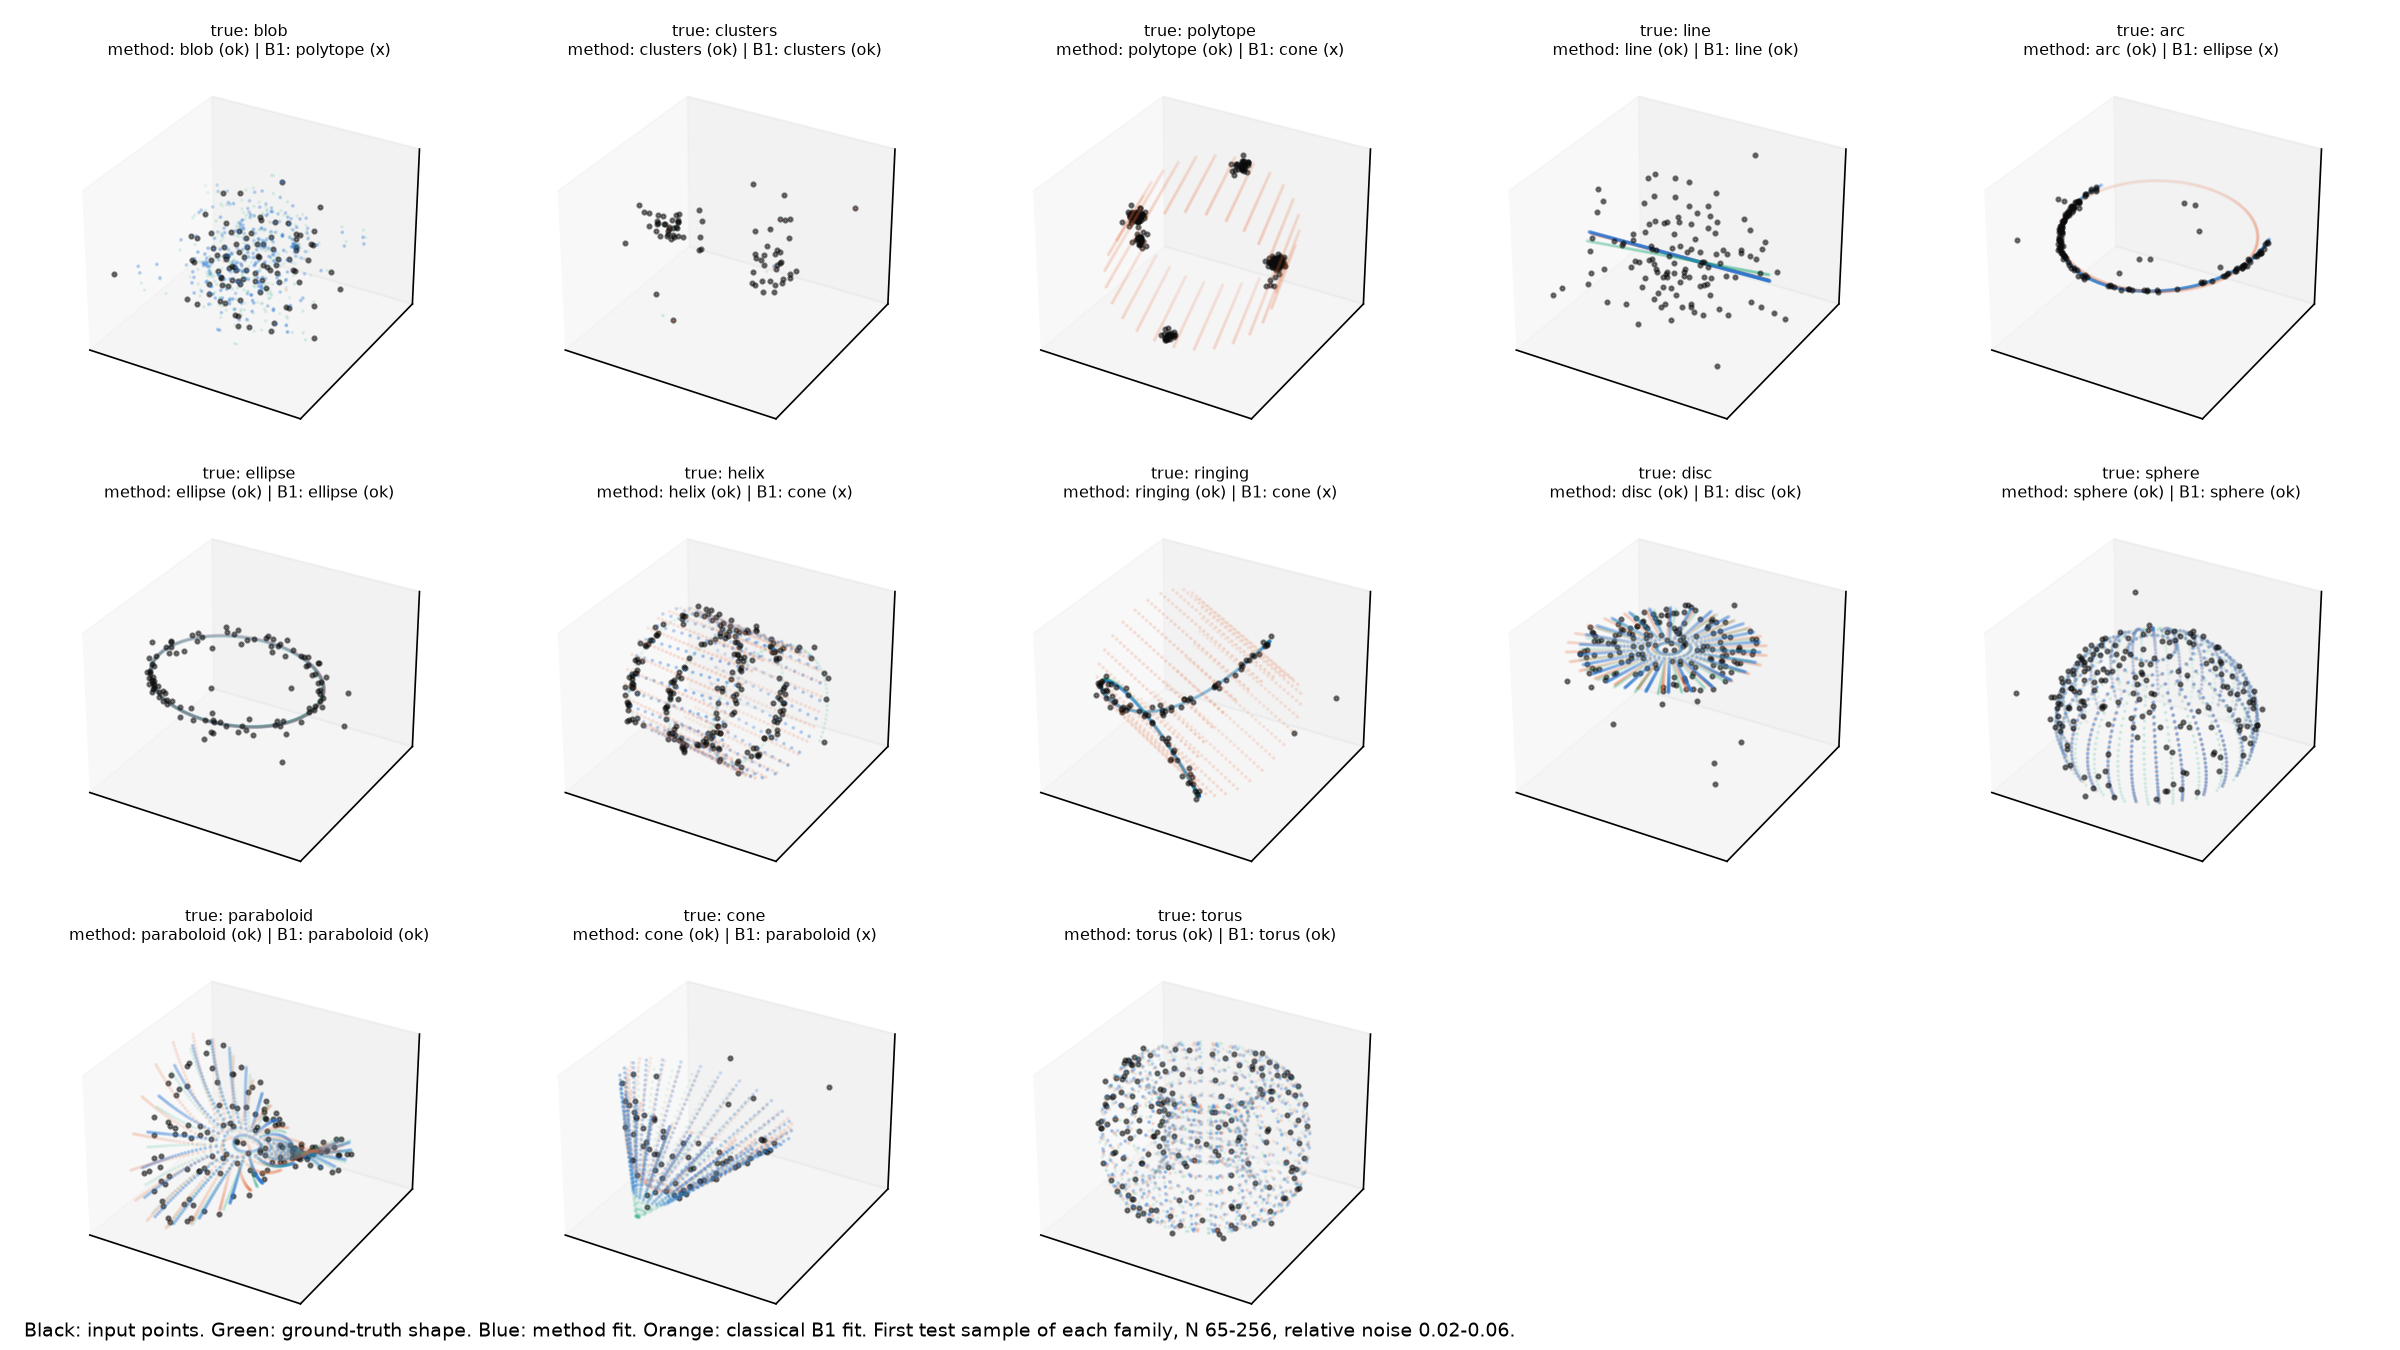
\includegraphics[width=\textwidth]{fig_gallery_synth.png}
\caption{The first synthetic test cloud of every family (65--256 points, relative noise 0.02--0.06): input points (black), ground-truth shape (green), method fit (blue), classical B1 fit (orange).}
\label{fig:gallery}
\end{figure}

\subsection{Real activations}
Table~\ref{tab:real} lists every real dataset and control, and Fig.~\ref{fig:real} shows the clouds with the fitted shapes. The coarse label agrees with the literature on \hthreeAgree{}/\hthreeN{} preregistered datasets; the label-permutation null gives $p=\hthreeP{}$, so \textbf{H3 is not supported} (it is not falsified either, since agreement is not below 50\%).

\paragraph{Successes.} The toy model of superposition with 6 features (R3) is labelled \fitRthreetmsnsix{} ($p=\pRthreetmsnsix{}$), with a fitted vertex on every feature direction (the octahedron of \citealp{elhage2022tms}). Llama's character-count manifold (R4) is labelled \fitRfourllamacounting{} ($p=\pRfourllamacounting{}$), a curve as in \citet{gurnee2025linebreaks}; under the preregistered rule a helix claim is not made because ringing is not rejected. Temperature (R8a) is labelled \fitReightallamatemperature{}, the arch PCA produces for a smoothly varying ordinal variable \citep{novembre2008horseshoe,antognini2018walks}, which agrees with the ``line'' of \citet{bhalla2026sae} at the coarse level. Colours (R7) are labelled \fitRsevenllamacolors{}, a curved surface as reported (paraboloid in \citealp{bhalla2026sae}).

\paragraph{Failures.} (i) GPT-2's positional embeddings (R1) are a 1D spiral whose radius varies along the curve; no family represents it (helix has constant radius, ringing three harmonics), and the classifier selects \fitRonegpttwowpos{} ($p=\pRonegpttwowpos{}$), a surface the spiral lies on. The held-out residual cannot reveal this error because held-out points also lie on the sphere. (ii) Weekdays and months (R5) form one tight cluster per token, 7 and 12 clusters, more than the 6 centroids the clusters family allows; the fitter threads a \fitRfiveallamaweekdays{} through them. (iii) Years (R6) and the grokked embeddings (R2) keep only \varRsixllamayears{} and \varRtwogrokkingWE{} of the variance in the top three components and are flagged ($\lambda_3/\lambda_4<1.5$): the 3D view cuts through a higher-dimensional structure, as expected for the several Fourier circles of a grokked model \citep{nanda2023progress}. (iv) Age (R8b) is a branching curve and true/false city statements (R9) two overlapping clouds of very different spread; both are outside the vocabulary (labelled \fitReightbllamaage{} and \fitRninellamatruthcities{}).

\begin{figure}[tbp]
\centering
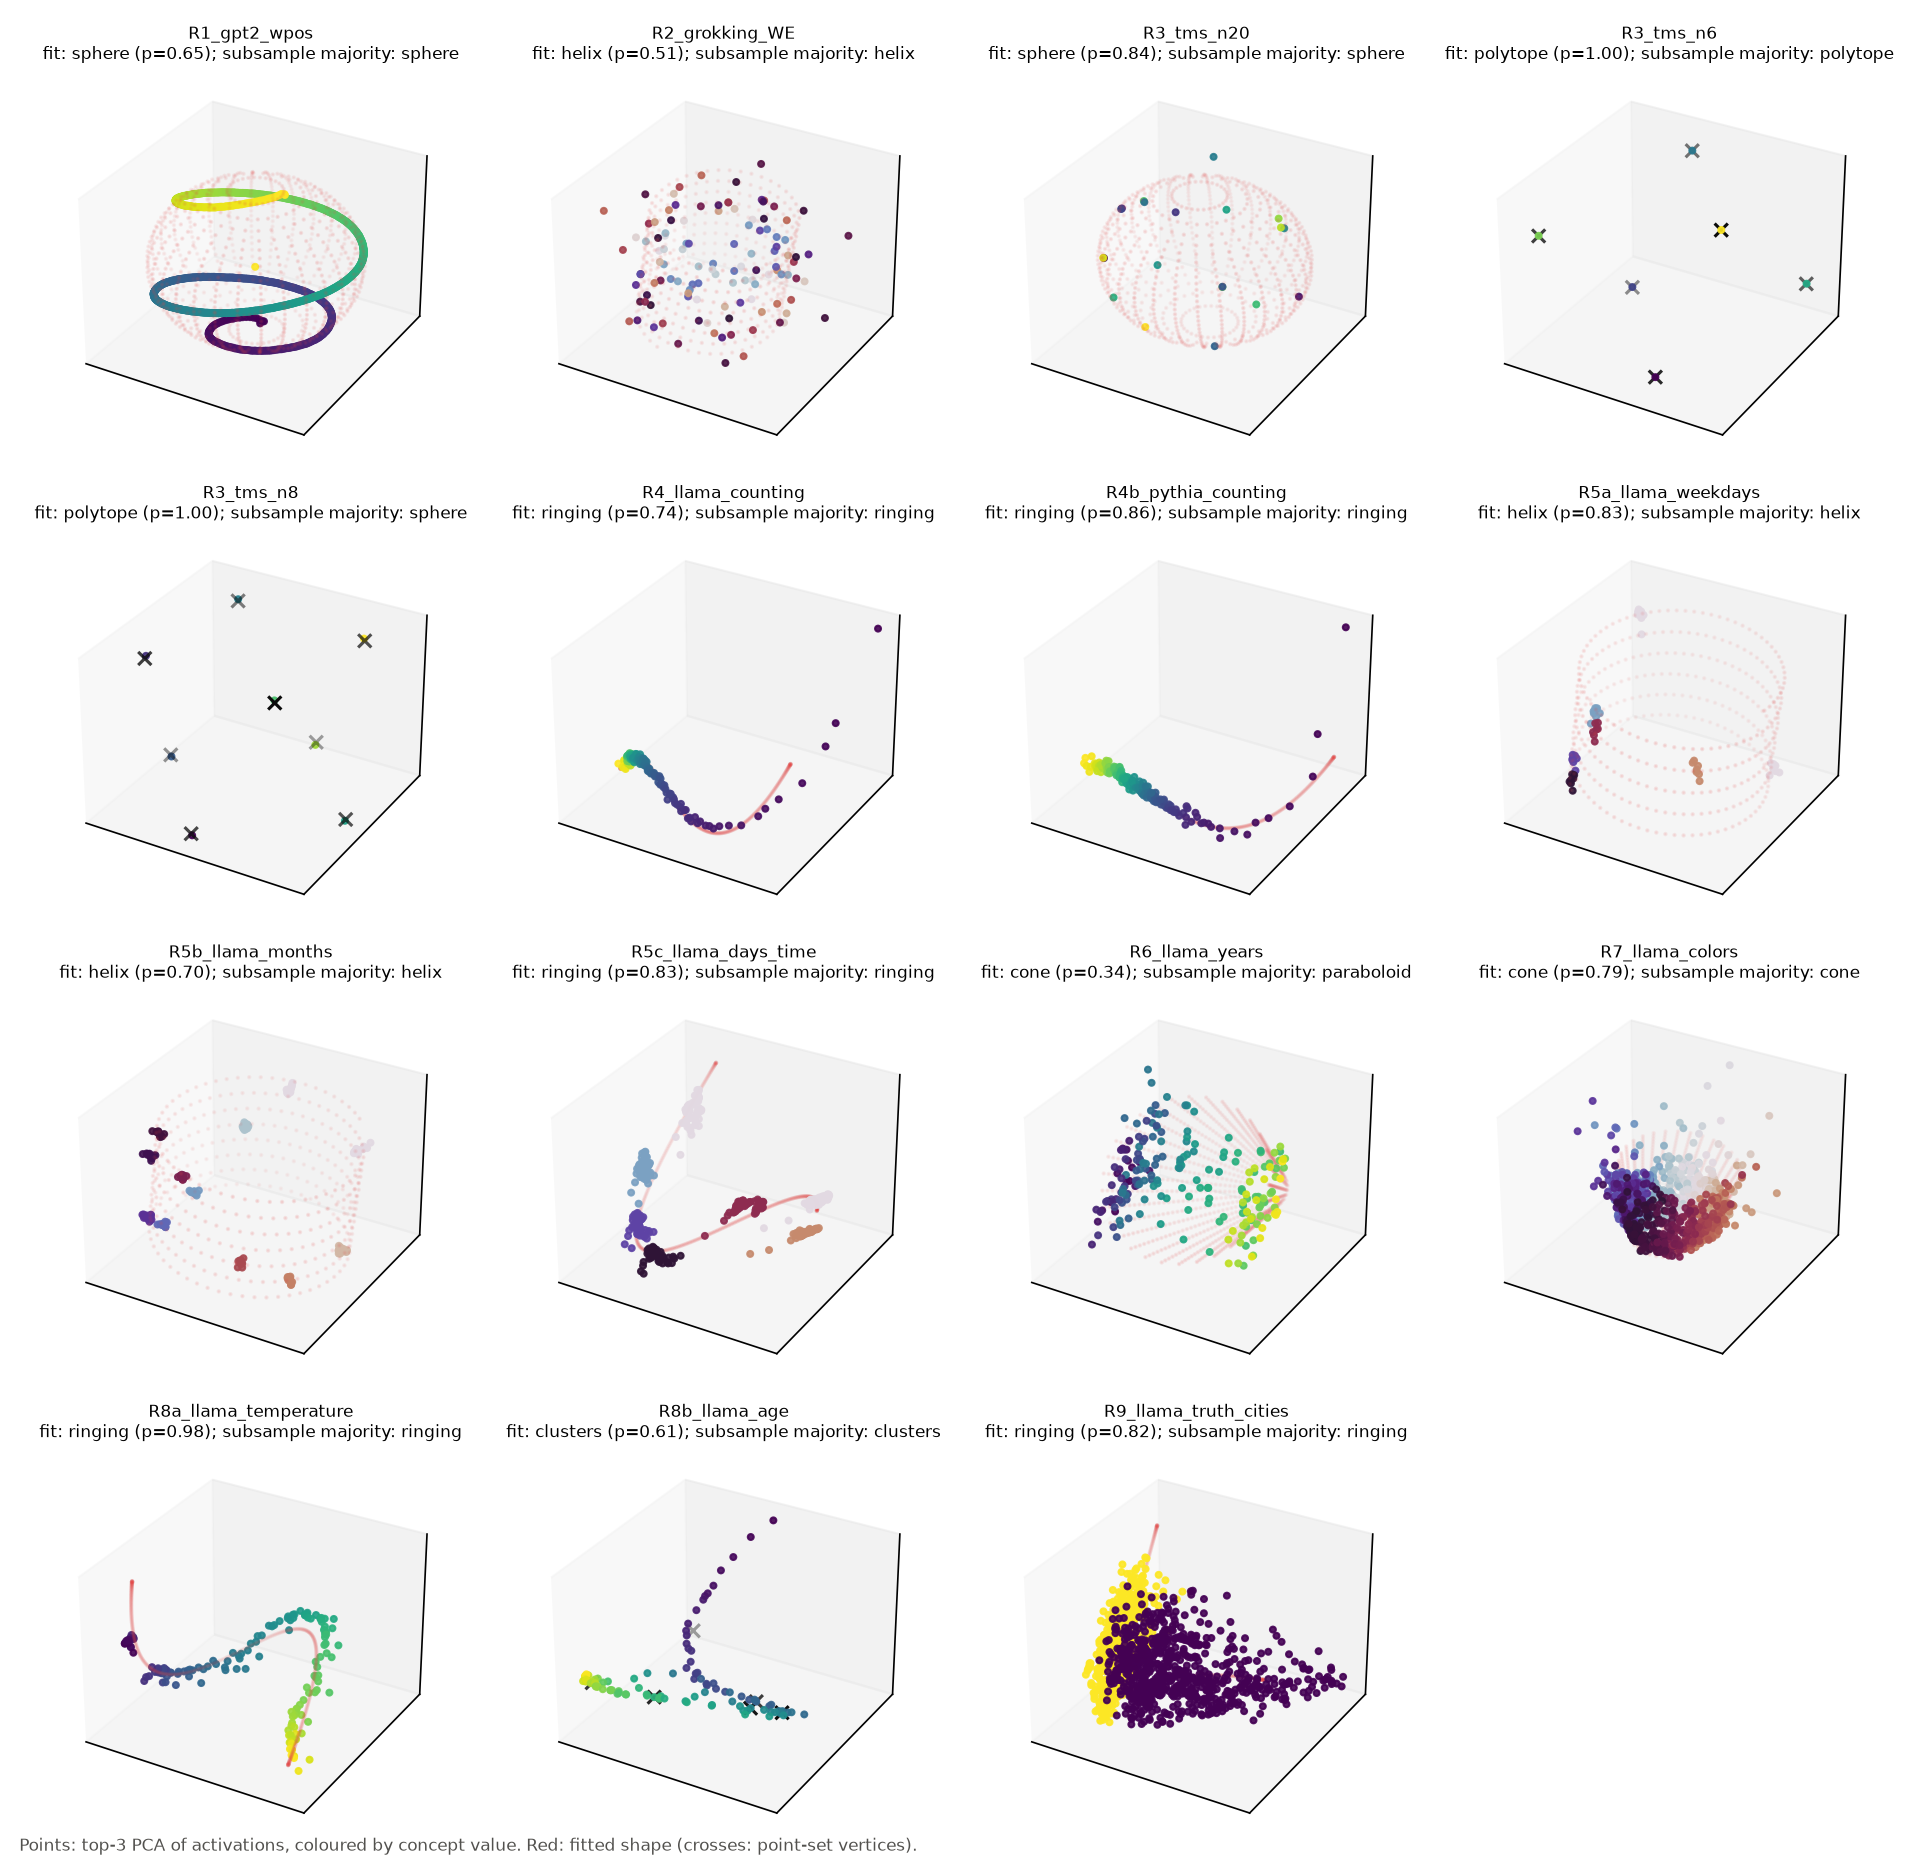
\includegraphics[width=\textwidth]{fig_real.png}
\caption{Real activation clouds in their top-3 PCA coordinates, coloured by concept value, with the fitted shape (red; crosses for point-set vertices). Titles give the full-cloud fit with its calibrated probability and the majority label over 200 random 80\% subsamples.}
\label{fig:real}
\end{figure}

\paragraph{Controls (H4).} Matched-covariance Gaussians are labelled blob in \hfourBlob{} of draws and the ordinal-process controls ringing in \hfourRing{} versus helix in \hfourHelix{}, so H4 passes as preregistered. A post-hoc split shows that this pass relies on the random walks (ringing in \hfourWalkRing{}): the smooth Gaussian-process controls alone are labelled helix in \hfourGpHelix{}. The classifier therefore confuses smooth ordinal processes with helices, the confound the preregistered helix rule guards against; for the fully evaluated Gaussian-process control the held-out residual favours ringing and the rule rejects the helix claim. Randomly initialised GPT-2 positional embeddings and grokking embeddings are labelled blob, but randomly initialised Llama is labelled \fitCthreellamamonthsinit{} for the month prompts: Fig.~\ref{fig:controls} shows genuine clusters, one per input token, because a random transformer still separates token identities. The preregistered expectation ``blob'' for this control was wrong, not the fitter.

\begin{figure}[tbp]
\centering
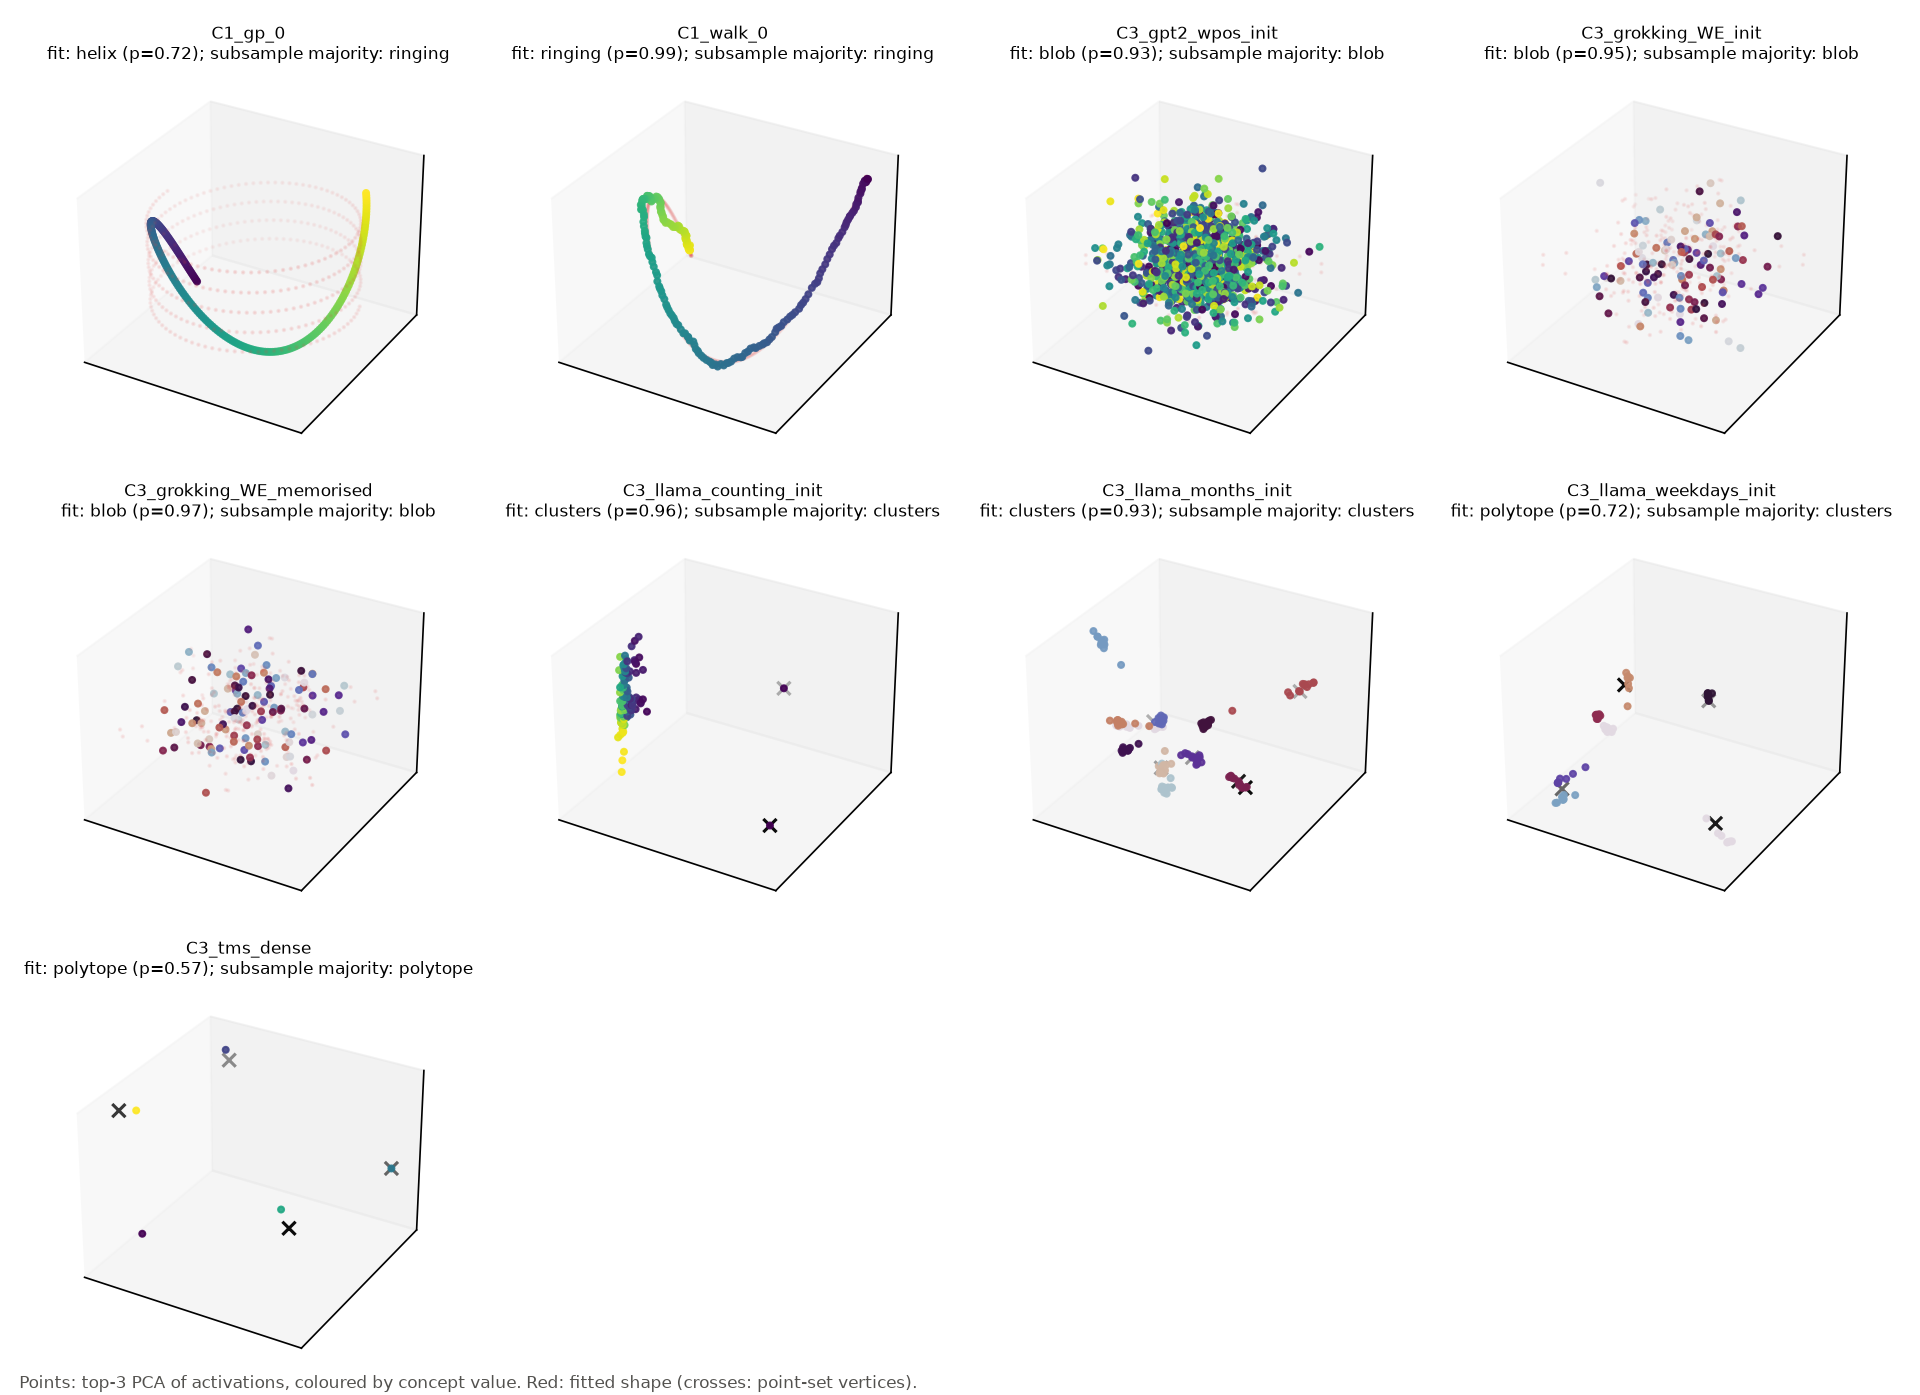
\includegraphics[width=\textwidth]{fig_controls.png}
\caption{Controls: a smooth Gaussian process and a random walk over an ordinal index (C1), and randomly initialised or untrained networks (C3).}
\label{fig:controls}
\end{figure}

\begin{sidewaystable}
\centering
\caption{Real datasets and controls (C1 shows the first of 10 draws of each process). Flags: $\lambda_3/\lambda_4<1.5$ (gap); OOD: residual above the synthetic 95th percentile of correct fits at that $N$. Held-out residuals, matched-Gaussian rates and model/layer details are in the full table in \texttt{reports/exp02\_real\_activations.md}.}
\label{tab:real}
\scriptsize
\begin{tabular}{llllllll}
\toprule
\textbf{Dataset} & \textbf{N x D} & \textbf{Top-3 var.} & \textbf{Expected (coarse / fine)} & \textbf{Fit (full cloud)} & \textbf{p} & \textbf{Subsample majority (freq.)} & \textbf{Flags} \\
\midrule
C1\_gp\_0 (prereg) & 200 x 768 & 99\% & 1d / ringing & helix & 0.72 & ringing (58\%) & - \\
C1\_walk\_0 (prereg) & 200 x 768 & 83\% & 1d / ringing & ringing & 0.99 & ringing (100\%) & - \\
C3\_gpt2\_wpos\_init (prereg) & 1023 x 768 & 1\% & 3d / blob & blob & 0.93 & blob (100\%) & gap$<$1.5 \\
C3\_grokking\_WE\_init (prereg) & 113 x 128 & 9\% & 3d / blob & blob & 0.95 & blob (100\%) & gap$<$1.5 \\
C3\_grokking\_WE\_memorised & 113 x 128 & 15\% & - / - & blob & 0.97 & blob (100\%) & gap$<$1.5 \\
C3\_llama\_counting\_init (prereg) & 150 x 4096 & 14\% & 3d / blob & clusters & 0.96 & clusters (98\%) & gap$<$1.5, OOD \\
C3\_llama\_months\_init (prereg) & 144 x 4096 & 19\% & 3d / blob & clusters & 0.93 & clusters (82\%) & gap$<$1.5, OOD \\
C3\_llama\_weekdays\_init (prereg) & 49 x 4096 & 34\% & 3d / blob & polytope & 0.72 & clusters (70\%) & gap$<$1.5, OOD \\
C3\_tms\_dense & 5 x 3 & 100\% & - / - & polytope & 0.57 & polytope (100\%) & - \\
R1\_gpt2\_wpos (prereg) & 1023 x 768 & 91\% & 1d / helix & sphere & 0.65 & sphere (74\%) & - \\
R2\_grokking\_WE (prereg) & 113 x 128 & 32\% & 1d / arc, ellipse & helix & 0.51 & helix (43\%) & gap$<$1.5 \\
R3\_tms\_n20 & 20 x 3 & 100\% & 0d / polytope, clusters & sphere & 0.84 & sphere (78\%) & - \\
R3\_tms\_n6 (prereg) & 6 x 3 & 100\% & 0d / polytope, clusters & polytope & 1.00 & polytope (100\%) & - \\
R3\_tms\_n8 (prereg) & 8 x 3 & 100\% & 0d / polytope, clusters & polytope & 1.00 & sphere (56\%) & - \\
R4\_llama\_counting (prereg) & 150 x 4096 & 69\% & 1d / helix & ringing & 0.74 & ringing (92\%) & - \\
R4b\_pythia\_counting & 150 x 1024 & 75\% & 1d / helix & ringing & 0.86 & ringing (100\%) & - \\
R5a\_llama\_weekdays (prereg) & 49 x 4096 & 66\% & 1d / arc & helix & 0.83 & helix (58\%) & gap$<$1.5 \\
R5a\_llama\_weekdays\_means (prereg) & 7 x 4096 & 78\% & 1d / arc & sphere & 0.40 & helix (74\%) & gap$<$1.5 \\
R5b\_llama\_months (prereg) & 144 x 4096 & 55\% & 1d / arc & helix & 0.70 & helix (87\%) & gap$<$1.5 \\
R5b\_llama\_months\_means (prereg) & 12 x 4096 & 60\% & 1d / arc & helix & 0.40 & helix (51\%) & gap$<$1.5 \\
R5c\_llama\_days\_time & 336 x 4096 & 58\% & 1d / arc & ringing & 0.83 & ringing (86\%) & gap$<$1.5 \\
R6\_llama\_years (prereg) & 199 x 4096 & 25\% & 1d / helix & cone & 0.34 & paraboloid (62\%) & gap$<$1.5 \\
R7\_llama\_colors (prereg) & 900 x 4096 & 66\% & 2d / paraboloid & cone & 0.79 & cone (83\%) & gap$<$1.5 \\
R8a\_llama\_temperature (prereg) & 150 x 4096 & 90\% & 1d / line & ringing & 0.98 & ringing (100\%) & - \\
R8b\_llama\_age (prereg) & 99 x 4096 & 85\% & 1d / line & clusters & 0.61 & clusters (96\%) & OOD \\
R9\_llama\_truth\_cities (prereg) & 1496 x 4096 & 53\% & 0d / clusters & ringing & 0.82 & ringing (100\%) & OOD \\
\bottomrule
\end{tabular}

\end{sidewaystable}
